\bisubsection{Antiphona marialis}{Marian antiphon}\pdfbookmark[section]{Antiphona marialis}{antiphona-marialis}

\vspace{-0.25cm}

\subsubsection{Alma Redemptoris}

\vspace{-0.25cm}

\bimusichangingdouble[A Dominica I Adventus usque ad Festum Baptismatis Domini inclusive:][From the 1st Sunday of Advent until the Feast of the Baptism of the Lord, inclusive:]{\gregorioscore{../MarianAntiphons/4694-an--alma_redemptoris_mater_(festivus_forma_ordinaria)--solesmes_2000s.gabc}}{Holy mother of our Redeemer, thou gate leading to heaven,
And star of the sea, help the falling people who seek to rise\,:\\
Thou who, all nature wondering, didst give birth to thy holy Creator.\\
Virgin always, hearing the greeting from Gabriel’s lips, take pity on sinners.}

\bimusichangingdouble[Vel, in tono simplici:][Or, in the simple tone:]{\gregorioscore{../MarianAntiphons/15264-an--alma_redemptoris--simplex.gabc}}{Holy mother of our Redeemer, thou gate leading to heaven,
And star of the sea, help the falling people who seek to rise\,:\\
Thou who, all nature wondering, didst give birth to thy holy Creator.\\
Virgin always, hearing the greeting from Gabriel’s lips, take pity on sinners.}

\subsubsection{Ave Regina cælorum}

\bimusichangingdouble[A Feria II Hebdomadæ I per annum uqsue ad Feriam IV Hebdomadæ Sanctæ, et post II Vesperas Sollemnitatis Assumptionis B. M. V. et in Memoria B. M. V. Reginæ:][From Monday of Week 1 through the year until Wednesday of Holy Week, and after Second Vespers of the Solemnity of the Assumptions of B. M. V. and on Memorials of B. M. V. the Queen:]{\gregorioscore{../MarianAntiphons/18754-an--ave_regina_caelorum--solesmes_2000s-simpler-neumes.gabc}}{Hail, Queen of heaven,\\
Hail Lady of the Angels\,:\\
Hail, root, hail the door,\\
Through which the Light of the world is risen\,:\\
Rejoice, glorious Virgin,\\
Beautiful above all\,:\\
Hail, O very fair one,\\
And plead for us to Christ.}
\bimusichangingdouble[Vel, in tono simplici:][Or, in the simple tone:]{\gregorioscore{../MarianAntiphons/15265-an--ave_regina_caelorum--simplex.gabc}}{Hail, Queen of heaven,\\
Hail Lady of the Angels\,:\\
Hail, root, hail the door,\\
Through which the Light of the world is risen\,:\\
Rejoice, glorious Virgin,\\
Beautiful above all\,:\\
Hail, O very fair one,\\
And plead for us to Christ.}

\newpage

\subsubsection{Regina cæli}
\vspace{-0.25cm}

\bimusichangingdouble[A Dominica Paschæ usque ad Dominicam Pentecostes:][From Easter Sunday until Pentecost Sunday:]{\gregorioscore{../MarianAntiphons/18753-an--regina_caeli--solesmes_2000s-simpler-neumes.gabc}}{Queen of heaven, rejoice, alleluia;\\
For He whom thou was chosen to bear, alleluia;\\
Has risen, as He said, alleluia;\\
Pray for us to God, alleluia.}

\bimusichangingdouble[Vel, in tono simplici:][Or, in the simple tone:]{\gregorioscore{../MarianAntiphons/15266-an--regina_caeli--simplex.gabc}}{Queen of heaven, rejoice, alleluia;\\
For He whom thou was chosen to bear, alleluia;\\
Has risen, as He said, alleluia;\\
Pray for us to God, alleluia.}

\vspace{-0.25cm}
\subsubsection{Salve Regina}
\vspace{-0.25cm}

\bimusichangingdouble[Post Dominicam Pentecostes:][After Pentecost Sunday:]{\gregorioscore{../MarianAntiphons/18654-an--salve_regina_(tono_solemnis)--solesmes_2000s.gabc}}{Hail holy queen, mother of mercy\,: \\
Hail our life, our sweetness, and our hope.\\
To thee do we cry, poor banished children of Eve.\\
To thee do we send up our sighs, mourning and weeping in this vale of tears.\\
Turn then most gracious advocate, thine eyes of mercy towards us.\\
And after this, our exile, show unto us the blessed fruit of thy womb, Jesus.\\
O clement\,: O loving\,: O sweet Virgin Mary.}

\bimusichangingdouble[Vel, in tono simplici:][Or, in the simple tone:]{\gregorioscore{../MarianAntiphons/18655-an--salve_regina_(tonus_simplici)--solesmes_2000s.gabc}}{Hail holy queen, mother of mercy\,: \\
Hail our life, our sweetness, and our hope.\\
To thee do we cry, poor banished children of Eve.\\
To thee do we send up our sighs, mourning and weeping in this vale of tears.\\
Turn then most gracious advocate, thine eyes of mercy towards us.\\
And after this, our exile, show unto us the blessed fruit of thy womb, Jesus.\\
O clement\,: O loving\,: O sweet Virgin Mary.}

\biinstruction{Tonus similis sollemni \textcolor{black}{Salve Regina} invenitur in Appendice, p. \textcolor{black}{\pageref{SalveAlt}.}}{A tone similar to the solemn \textcolor{black}{Salve Regina} tone is found in the Appendix, p. \textcolor{black}{\pageref{SalveAlt}.}}

\subsubsection{Sub tuum præsidium}

\bimusichangingdouble[Post I Vesperas Sollemnitatum, extra Tempus Paschale:][After 1st Vespers of Solemnities, outside Easter Time:]{\gregorioscore{../MarianAntiphons/18652-an--sub_tuum_praesidium--solesmes_2000s.gabc}}{We fly to thy patronage, O holy Mother of God\,:\\
despise not our prayers in our necessities\,:\\
but deliver us from all dangers,\\
O ever glorious and blessed Virgin.}

\vfill
\begin{center}
  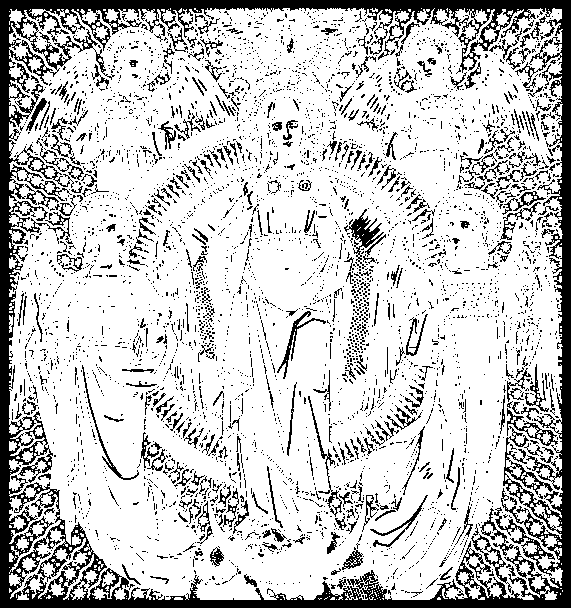
\includegraphics[width=0.44\textwidth]{../Images/Mary.pdf}
\end{center}
\vfill
